\section{From a fixed cross kernel to product sampling}\label{sec:universality}
This section proves Theorem~\ref{thm:universal} by coupling the actual processes.
Internal sampling first forgets a random label transposition under a dispersion
bound. This controls the whole cross load-pair table.
A sorted-rank coupling then uses greedy nonexpansion.
Fix $\theta=1/200$, $K_0=16/3$, and $I=(1-\eps)/2$.
The constants are conservative.

\begin{figure}[t]
\centering
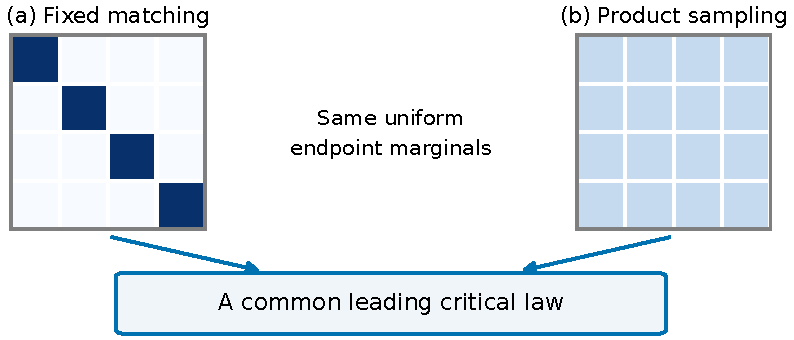
\includegraphics[width=\textwidth]{figures/kernel_universality.pdf}
\caption{Different fixed cross correlations share the critical law under the
model and scaling of Theorems~\ref{thm:universal}--\ref{thm:limit}.
The grids show conditional candidate-pair probabilities in one cross direction,
with four illustrative labels on each side. Matching probabilities are $1/4$
on the diagonal and zero elsewhere; product probabilities are all $1/16$.
Both have uniform marginals. Internal sampling and rare cross arrivals are
essential to the theorem; uniform marginals alone do not imply independent loads.}
\label{fig:kernels}
\end{figure}

\begin{lemma}[Dispersion]\label{lem:moment}
With $\xi_v=A_v-M_{s(v)}/q$ and $\Gamma=\sum_v\cosh(\theta\xi_v)$, every fixed uniform-marginal kernel satisfies
\begin{equation}\label{eq:moment}
 \sup_{n\ge0}\E\Gamma_n\le K_0q.
\end{equation}
\end{lemma}
\begin{proof}
The rank-based potential argument is given in Supplement
section~\ref*{app:dispersion}. It uses only the cross marginals.
\end{proof}

\begin{lemma}[Random transposition]\label{lem:swap}
Let $\mu_n$ be the law of the actual fixed-kernel configuration. Independently choose two uniform labels $i,j$ in one side, and let $\tau$ swap them. For $\ell\ge4$, integer $L=q\ell$, and $n\ge L$,
\begin{align}
 \E_{i,j}\TV(\mu_n,\tau\mu_n)&\le\eta,\label{eq:eta}\\
 \eta&=\min\left\{1,\frac{32K_0}{\theta\sqrt\ell}
 +16K_0e^{-\theta\ell/16}+e^{-L/48}+4\eps\ell\right\}.\nonumber
\end{align}
\end{lemma}
\begin{proof}
Compare the original and transposed configurations through the conjugate
kernel. The two discrepancies behave as tags until they meet.
Suppress cross events touching a tag; internal updates then make the tag gap
no harder to absorb than a fair walk. Dispersion controls the initial gap
and deviations at the window endpoints. On the remaining event, nonmeeting
requires at least $\lceil\ell/4\rceil$ embedded jumps.
A fixed-jump reflection bound gives the first term of $\eta$.
The conjugate-kernel comparison adds a second cross-touch allowance.
Supplement section~\ref*{app:swapdetails} gives the full coupling and constants;
it does not condition a martingale estimate on a future jump count.
\end{proof}

For one cross direction write $Q_n$ for its actual conditional joint load-pair law and $p_n,r_n$ for the empirical side marginals. If $0\le f\le1$, define
\[
 C_B(f)=\frac1m\sum_{ij}B_{ij}f(U_i,V_j)
       -\frac1{m^2}\sum_{ij}f(U_i,V_j).
\]
The test may use parameters unchanged by the side swap, including community
means. Let $I_0$ be uniform, draw $J_0\mid I_0$ from the corresponding row
of $B$, and draw $J'_0$ independently and uniformly. We claim
\begin{equation}\label{eq:correlation}
 \E C_B(f)^2\le2\eta+2/m,
 \qquad \E|C_B(f)|\le\sqrt{2\eta+2/m}.
\end{equation}
Write $C=C_B(f)$ and take these auxiliary indices independently of the
configuration. Pointwise,
\[
 C^2=\E_{\rm aux}\bigl[C\{f(U_{I_0},V_{J_0})-f(U_{I_0},V_{J'_0})\}\bigr].
\]
For fixed indices let $\tau$ exchange $J_0,J'_0$. The product-marginal term of $C$ is unchanged, and $|C(\tau A)-C(A)|\le2/m$. Apply total variation to $G(A)=C(A)f(U_{I_0},V_{J_0})$, for which $|G|\le1$. Thus the expected difference is at most $2\TV(\mu_n,\tau\mu_n)+2/m$. After averaging, $(J_0,J'_0)$ are independent uniform side labels: column sums make $J_0$ uniform, even though it depends on $I_0$. Lemma~\ref{lem:swap} gives \eqref{eq:correlation}. The bounded-test TV cost is $2\eta$. This controls the second moment, rather than only a signed average.

Center each load coordinate at its community's integer mean part. For each fixed offset cell in $[-R,R]^2$, its indicator satisfies \eqref{eq:correlation}. Summing over this deterministic square and using \eqref{eq:moment} outside it yields
\begin{equation}\label{eq:rho}
 \E\norm{Q_n-p_n\otimes r_n}_1\le\rho,
 \quad \rho=\min\{2,(2R+1)^2\sqrt{2\eta+2/m}
                      +16K_0e^{-\theta(R-1)}\}.
\end{equation}
Indeed $Q$ and the product have the same marginals; twice their marginal tail masses bounds the mass outside the square. Replacing the mean by its integer part costs at most one in the exponential bound. No supremum over arbitrary data-dependent tests is taken.

It remains to compare two actual process laws. Sort each side separately. Integer greedy updates using the same offered ranks are nonexpansive in sorted $\ell_1$ distance: if different winners are chosen, the two relevant coordinate differences have the ordering needed for their $+1,-1$ changes not to increase the absolute sum; sorting again minimizes the matching cost. Internally use common independent uniform ranks. At a cross, sample the actual fixed edge in the fixed process, then maximally couple its load pair from $Q_F$ to a virtual pair from $p_F\otimes r_F$. Given the virtual loads, choose ranks independently and uniformly inside the equal-load blocks. Conditional on the entire joint past before drawing the current edge, these ranks are independent uniforms, since a block of size $k$ has mass $k/m$ followed by probability $1/k$ per rank. Use the same ranks in the product process, which therefore has its genuine transition law. Independence need not persist after additionally conditioning on the current realized fixed edge.

On successful load-pair coupling the actual and virtual sorted fixed-process updates agree, including ties. On failure their distance is at most two. Hence
\[
 \mathcal D_{n+1}\le\mathcal D_n+
 2\one_{\{\text{cross and load-pair coupling fails}\}}.
\]
Before $L$ use failure probability one; afterwards its expected conditional value is at most $\rho/2$. Summing the nonnegative counts gives the explicit bound
\begin{equation}\label{eq:finitecoupling}
 \E\max_{n\le N}\mathcal D_n
 \le2\eps\min(N,L)+\eps\rho(N-L)_+.
\end{equation}
Take $\ell=\max(4,\lceil q^{2/3}\rceil)$ and $R=\lceil(2/\theta)\log q\rceil+1$. Then \eqref{eq:finitecoupling} divided by $q$, for $N\le Tq^2$, is $O(q^{-1/6}\log^2q)$. Both the community difference and every positive-part sum are $1$-Lipschitz in sorted load distance. This proves Theorem~\ref{thm:universal}. The bound is asymptotic and extremely conservative; it is not a numerical error bar at the experimental sizes.
